\section{Extensions}\label{sec:extension}

The WAIT and Nested WAIT algorithms assume constant arrival rates and a fixed number of segments matching the number of prompt types. In practice, however, LLM inference systems face two additional challenges: (i) \textbf{time-varying workloads}, where arrival rates fluctuate over time; (ii) \textbf{numerous prompt types}, where maintaining separate thresholds for hundreds of output lengths becomes infeasible. We address these challenges through two extensions that preserve the core algorithmic principles---eviction prevention and approaching load balance---while adapting the threshold construction to more realistic deployment settings.

First, we extend Nested WAIT to handle time-varying arrival rates $\lambda_j^t$ by replacing constant-rate threshold conditions with accumulated arrival constraints over each iteration window. This gives a conservative finite-horizon guarantee under bounded window loads. The delay bound additionally requires that the first threshold can be collected on the service-normalized time scale, which rules out arbitrarily long low-arrival intervals (Section~\ref{sec:time_varying}). Second, we introduce a \textbf{segment-wise design} that groups many prompt types into a smaller number of decode-stage segments, reducing algorithmic complexity while maintaining the same threshold structure (Section~\ref{sec:segment_design}).

\subsection{Time-Varying Arrival Rates}\label{sec:time_varying}

Time-varying arrival rates capture moderate changes in workload intensity, such as predictable daily variation or slowly changing demand. The threshold mechanism remains valid when the accumulated arrivals during each service window stay below the corresponding completion capacity. Formally, we replace constant rates $\lambda_j$ with time-dependent rates $\lambda_j^t$, assumed continuous and uniformly bounded by $\lambda_{\max} < \infty$ to prevent unbounded bursts.

We analyze the asymptotic optimality of the Nested WAIT algorithm under time-varying arrival rates, denoted $\lambda_j^t$ for prompt type $j \in [m]$ at physical time $t \in [0, T]$.

For a service-normalized window \(h\), define the expected number of type-\(j\) arrivals in the corresponding physical interval by
\[
    \mathcal A_j^{(\zeta)}(t,h)
    :=
    \zeta\int_t^{\min\{T,t+h/\zeta\}}\lambda_j^u\,du .
\]
The truncation only affects the final partial window and can only reduce the number of arrivals.
Recall from Equation \eqref{eq:wait_thresholds} that $\Delta T_{[1,2,\dots,m]}(n_1,\cdots,n_m)$ represents the service-normalized iteration cost when processing exactly $n_k$ prompts at each stage in segment $k$, for all $k \in [m]$, as in \eqref{eq:nested_wait_thresholds}, where $n_k$ is the threshold defined in Algorithm \ref{alg:nested_wait}.

For the Nested WAIT policy defined by $\pi = [n_1, \dots, n_m]$, we impose the following uniform slack conditions for all $t\in [0, T]$, $0<h\leq \Delta T_{[1,2,\cdots,m]}(n_1,\cdots,n_m)$ and $k = 1, 2, \dots, m-1$, analogous to \eqref{eq:nested_wait_thresholds}:
\begin{equation}
    \label{eq:nested_wait_thresholds_time_varying}
\begin{aligned}
        & \sum_{j=1}^m \mathcal A_j^{(\zeta)}(t,h)
        \leq
        \sum_{j=1}^m \mathcal A_j^{(\zeta)}\!\left(t,\Delta T_{[1,2,\cdots,m]}(n_1,\cdots,n_m)\right)< n_1, \\
        & p_k^{(\zeta)}(t,h) < n_k/n_{k-1} < 1,\quad k=2,\dots,m,
    % & n_{k+1} \sum_{j=k}^m \lambda_j\big[t, t + \Delta t \big]  > n_k \sum_{j=k+1}^m \lambda_j\big[t, t + \Delta t \big],.
\end{aligned}
\end{equation}
where \(p_k^{(\zeta)}(t,h)=(\sum_{j=k}^m\mathcal A_j^{(\zeta)}(t,h))/(\sum_{j=k-1}^m\mathcal A_j^{(\zeta)}(t,h))\) when the denominator is positive, and \(p_k^{(\zeta)}(t,h)=0\) otherwise. The time-varying fluid benchmark is
\[
    \throughput_T^*
    :=
    \frac{1}{T}\int_0^T\sum_{j=1}^m\lambda_j^t l_j'\,dt .
\]
For the downstream safety buffers, set
\[
    p_k^*
    :=
    \sup_{\substack{t\in[0,T],\,0<h\le \Delta T_{[1,\dots,m]}\\
    \sum_{j=k-1}^m\mathcal A_j^{(\zeta)}(t,h)>0}}
    \frac{\sum_{j=k}^m\mathcal A_j^{(\zeta)}(t,h)}
    {\sum_{j=k-1}^m\mathcal A_j^{(\zeta)}(t,h)},\qquad k\ge2,
\]
and set \(p_k^*=0\) if the denominator is zero for all such windows.
Segments with \(p_k^*=0\) have no stochastic downstream input and can be omitted or merged; the theorem below is stated for downstream segments with \(p_k^*>0\).
\paragraph{First-segment waiting.}
The window-load conditions above control overload and downstream boundary queues. A delay guarantee also needs a mild lower-side condition: if arrivals nearly stop, a subthreshold first-segment queue can wait for a long physical time before the next batch forms. Let \(\tau_1^{(\zeta)}(t)\) be the physical time needed, starting at time \(t\), for the scaled aggregate external arrival process to generate \(n_1\) arrivals. For the \(O(1)\) service-normalized delay bound below, assume there is a constant \(H<\infty\), independent of \((\zeta,T)\), such that
\[
    \sup_{t\in[0,T]}\zeta\,\mathbb E[\tau_1^{(\zeta)}(t)]\le H .
\]
This condition is implied, for example, by a uniform lower bound \(\sum_{j=1}^m\lambda_j^t\ge\lambda_{\min}>0\). Without such a condition, the throughput and memory statements remain meaningful, but the service-normalized delay can be dominated by waiting through a long low-arrival interval.
The following theorem extends Theorem~\ref{thm:nested_wait_heavy_traffic} to time-varying arrival rates.

\begin{theorem}
\label{thm:nested_wait_heavy_traffic_time_varying}
Suppose the thresholds $\pi = [n_1, \dots, n_m]$ satisfy \eqref{eq:nested_wait_thresholds_time_varying} and the physical memory capacity \(C\) fulfills:
\[
\begin{aligned}
	C &\ge M_{\mathrm{req},\mathrm{tv}}^{(\zeta,\pi)}
	:= M^{\pi} + \sum_{k=2}^m (l + l_{k-1}') \left(n_k + \theta_k^{-1} \ln\!\left( \tfrac{m(1+\zeta T/d_0)}{\delta} \right)\right) \\
	    &= O\!\left( M^\pi + \sum_{k=2}^m \theta_k^{-1}  (l + l_{k-1}') \ln\!\left( \tfrac{m(1+\zeta T/d_0)}{\delta} \right) \right),
\end{aligned}
\]
where the memory usage $M^\pi$ is defined as \eqref{eq:nested_wait_memory} and \(\theta_k>0\) is the unique solution of
\[
    e^{-\theta_k n_k}(1-p_k^*+p_k^*e^{\theta_k})^{n_{k-1}}=1,
\]
with lower bound \(\theta_k\ge 8(n_k-n_{k-1}p_k^*)/n_{k-1}\).
All quantities \(p_k^*\), \(\theta_k\), and \(M_{\mathrm{req},\mathrm{tv}}^{(\zeta,\pi)}\) are evaluated for the given scaled finite-horizon system \((\zeta,T)\).
For the corresponding no-overflow Nested WAIT dynamics,
$$
    \begin{aligned}
        &\throughput_T^* - \mathbb{E}\left[ \throughput^{(\zeta, \pi)} \right]
   = O\left( (\zeta T)^{-1} \right).
    \end{aligned}
$$
Additionally, the no-overflow dynamics are feasible on the physical GPU, i.e., memory usage remains below \(C\), with probability at least $1 - \delta$ over the time horizon $[0,T].$
If the first-segment waiting condition above also holds, then the service-normalized delay metrics satisfy
\[
\mathbb{E}\left[ \Latency^{(\zeta, \pi)} \right], \,\mathbb{E}\left[ \TTFT^{(\zeta, \pi)} \right] = O(1).
\]
\end{theorem}

The extension to time-varying rates preserves the dimensionality reduction structure from Theorem~\ref{thm:nested_wait_heavy_traffic}. The key adaptation is that threshold conditions~\eqref{eq:nested_wait_thresholds_time_varying} must hold uniformly over physical time \(t \in[0,T]\), replacing constant-rate arrival counts with the scaled-window arrivals \(\mathcal A_j^{(\zeta)}(t,h)\) over each service-normalized iteration window. These upper-side conditions control overload and memory growth. The separate first-segment waiting condition controls the time needed for the Segment 1 entry queue to reach its threshold. For downstream segments, prompts transitioning from segment \(k-1\) to segment \(k\) are controlled by the corresponding time-varying thinning probability. The Lindley recursion and Doob's maximal inequality apply with worst-case arrival and thinning parameters, bounding queue lengths with the same logarithmic overhead. Appendix~\ref{appendix:: proof of nested optimality, time varying.} provides the detailed proof.

\subsection{Segment Design}\label{sec:segment_design}

When LLM systems handle many distinct output lengths, maintaining individual thresholds for each type becomes impractical: the algorithm must track queue lengths separately for every output length, increasing memory overhead and implementation complexity. The \textbf{segment-wise design} addresses this by grouping similar output lengths into $L \leq m$ segments, where each segment $k$ aggregates types with comparable decode lengths. This reduces algorithmic complexity from $O(m)$ to $O(L)$ while preserving the threshold logic: prompts still classify themselves on the fly, but now at segment boundaries rather than individual type boundaries.

We assume constant arrival rates for clarity, though the approach extends to time-varying rates as discussed in Section~\ref{sec:time_varying}. Consider $m$ prompt types with decode lengths $l_1' < \cdots < l_m'$ and arrival rates $\lambda_1, \lambda_2, \cdots, \lambda_m$. Our objective is to merge these into $L$ ordered segments, where $L \leq m$. Choose cut points \(0=h_0<h_1<\cdots<h_L=m\), so segment \(k\) contains output-length classes \(h_{k-1}+1,\ldots,h_k\).

For each segment $k \in \{1, \dots, L\}$, the total arrival rate is defined as $\lambda_k' = \sum_{h_{k-1}< j\le h_k} \lambda_j$. Additionally, we define $\lambda'(k_1 \to k_2) := \sum_{r=k_1}^{k_2} \lambda_r'$ for $1 \leq k_1 \leq k_2 \leq L$.

Given a policy $\pi=[n_1,\dots,n_L]$ with threshold $n_k$ for the $k$-th segment in Algorithm \ref{alg:nested_wait}, we formulate a linear system analogous to Equation \eqref{eq:nested_wait_thresholds}:
\begin{equation}          \label{eq:nested_wait_thresholds_L}
    \begin{aligned}
    &\Delta T_{[1:L]}(n_{1:L}) < \frac{n_1}{\sum_{r=1}^L \lambda_r'},  \\
    &p_k < \frac{n_k}{n_{k-1}} < 1,\quad \forall k=2,\dots,L,
    \end{aligned}
\end{equation}
where $p_k =\frac{\lambda'(k \to L)}{\lambda'(k-1 \to L)}$ for \(k\ge2\). The strict first inequality gives negative drift for the first segment's entry queue, which is needed for the \(O((\zeta T)^{-1})\) throughput gap and \(O(1)\) service-normalized delay in Theorem~\ref{thm:nested_wait_heavy_traffic, any segment}. Let \(r_k=l_{h_k}'\) be the decode boundary of segment \(k\), with \(r_0=0\). Define \(\delta_1=r_1+1\), \(\bar s_1=r_1/2\), and for \(k\ge2\), \(\delta_k=r_k-r_{k-1}\) and \(\bar s_k=(r_{k-1}+1+r_k)/2\). Then \(\Delta T_{[1,\dots,L]}(n_1,\dots,n_L)=d_0+d_1M^\pi(n_1,\dots,n_L)\), where the base memory used by threshold-sized segment batches is
\[
M^{\pi}(n_1, \dots, n_L) = \sum_{k=1}^L n_k (l+\bar s_k)\delta_k.
\]
For heterogeneous prefill lengths, the segment logic is unchanged because boundaries are determined by decode progress. A sufficient memory condition replaces the common \(l\) in each segment by a segment-wise upper bound \(\bar l_k=\max\{l_j: \text{output-length class }j\text{ can enter segment }k\}\), or by the corresponding class-weighted term when the output-length mix within the segment is known.

The segment-wise design achieves two practical goals: (i) \textbf{robustness} to varying or uncertain type distributions---if actual output lengths differ slightly from predictions, grouping into segments absorbs the variation; and (ii) \textbf{simplicity} in deployment---the scheduler maintains thresholds for a small number of decode-stage segments rather than for every possible output length. The theoretical guarantee shows that this simplification preserves the same asymptotic throughput rate, with the same logarithmic safety-buffer structure.

\begin{theorem}
\label{thm:nested_wait_heavy_traffic, any segment}
For any fixed number of segments $L$ and thresholds $\pi = [n_1, \dots, n_L]$ satisfying Equation \eqref{eq:nested_wait_thresholds_L}, if the physical memory capacity \(C\) satisfies:
\begin{equation}
    \label{eq:nested_wait_memory_L}
    \begin{aligned}
	C &\ge M_{\mathrm{req},L}^{(\zeta,\pi)}
	:= M^\pi
		+ \sum_{k=2}^L (l + r_{k-1}) n_k \\
	&\quad
	+ \sum_{k=2}^L (l + r_{k-1}) \theta_k^{-1}
\ln\left( \frac{m(1+\zeta T/d_0)}{\delta} \right) \\
&= O\biggl( M^\pi
+ \sum_{k=2}^L (l + r_{k-1}) \theta_k^{-1}
\ln\left( \frac{m(1+\zeta T/d_0)}{\delta} \right) \biggr),
    \end{aligned}
\end{equation}
where $\theta_k>0$ is the unique solution of \(e^{-\theta_k n_k}(1-p_k+p_ke^{\theta_k})^{n_{k-1}}=1\), with lower bound $8(n_k-n_{k-1}p_k)/n_{k-1}$ for \(k\ge2\). The logarithm uses \(m\) as a conservative upper bound on the number of segment boundaries, since \(L\le m\).
For the corresponding no-overflow Nested WAIT dynamics, the performance satisfies:
$$\throughput^* - \mathbb{E}\left[ \throughput^{(\zeta, \pi)} \right] = O\left( (\zeta T)^{-1} \right),$$
$$\mathbb{E}\left[ \Latency^{(\zeta, \pi)} \right] = O(1),$$
$$\mathbb{E}\left[ \TTFT^{(\zeta, \pi)} \right] = O(1).$$
Moreover, the no-overflow dynamics are feasible on the physical GPU, i.e., memory is not exceeded, with probability at least \( 1 - \delta \) over the time horizon \(t \in [0,T]\).
% , where the total time horizon $T=\sum_{i=1}^S \Delta T_{i\text{-th Batch}}\geq S\cdot \min \Delta T_{\text{Batch}}$.
\end{theorem}

\paragraph{Proof of Theorem~\ref{thm:nested_wait_heavy_traffic, any segment}.}
The proof applies the Nested WAIT argument in Appendix~\ref{appendix::proof of nested_wait_heavy_traffic} to aggregated segment classes. The only changes are the segment arrival rates and the segment boundaries; the boundary-thinning domination, Lindley bound for downstream boundary queues, and high-probability martingale buffer are the same as in Theorem~\ref{thm:nested_wait_heavy_traffic}. Segment \(k\) contains original output-length classes with aggregate rate \(\lambda_k'=\sum_{h_{k-1}<j\le h_k}\lambda_j\), and the rate of prompts that can reach segment \(k\) is \(\lambda'(k\to L)=\sum_{r=k}^L\lambda_r'\). Hence, conditional on a threshold-sized cohort crossing boundary \(r_{k-1}\), the number of prompts that continue to segment \(k\) is dominated by a binomial random variable with parameters \(n_{k-1}\) and \(p_k=\lambda'(k\to L)/\lambda'(k-1\to L)\), exactly as in the boundary-thinning step of Theorem~\ref{thm:nested_wait_heavy_traffic}. The threshold conditions in \eqref{eq:nested_wait_thresholds_L} give negative drift for the Segment 1 entry queue and for every downstream boundary queue. Therefore the same Lindley-recursion bounds give uniformly bounded expected entry and boundary queues. The terminal-work and time-average queue conversions used in Appendix~\ref{appendix::proof of nested_wait_heavy_traffic} then yield the \(O((\zeta T)^{-1})\) normalized throughput gap and \(O(1)\) service-normalized latency and TTFT bounds.

It remains to check memory. The base term \(M^\pi=\sum_{k=1}^L n_k(l+\bar s_k)\delta_k\) charges the threshold-controlled interior stages of each segment. The resident boundary queue at \(r_{k-1}\), \(k\ge2\), is treated separately, with deterministic component \(n_k(l+r_{k-1})\) and stochastic carryover controlled by the exponential-martingale bound used in Appendix~\ref{appendix_lemma::proof of solution to martingale exists}. Applying that bound over at most \(1+\zeta T/d_0\) processing opportunities and union bounding over downstream segment boundaries gives the logarithmic buffer in \eqref{eq:nested_wait_memory_L}. Since \(L\le m\), using \(m\) in the logarithm is conservative. On this high-probability event, the no-overflow Nested WAIT dynamics are feasible whenever \(C\ge M_{\mathrm{req},L}^{(\zeta,\pi)}\), completing the proof.

We validate the segment-wise design numerically using a real-data workload derived from the \texttt{lmsys-chat-1m} dataset~\cite{zheng2023lmsys} (Section~\ref{sec:experiments}). Decode lengths range up to 500 tokens in this workload, and the segment arrival rates are proportional to the empirical frequencies of requests whose output lengths fall in the corresponding decode-stage ranges.

We analyze the three components of the memory bound in Equation \eqref{eq:nested_wait_memory_L}: (1) the base batch memory \(M^\pi=\sum_{k=1}^L n_k(l+\bar s_k)\delta_k\), (2) the deterministic boundary-queue term \(\sum_{k=2}^L n_k(l+r_{k-1})\), and (3) the high-probability boundary-queue term \(\sum_{k=2}^L \theta_k^{-1}(l+r_{k-1})\ln\!\left( \frac{m(1+\zeta T/d_0)}{\delta} \right)\).

Figures \ref{fig:fixed_T_200_rate_50_delta_0.1_1e-5}, \ref{fig:fixed_T_200_rate_500_delta_0.1_1e-5}, and \ref{fig:fixed_delta_0.001_rate_50_T_20_2000} plot these three memory components (y-axis) as functions of the number of segments $L$ (x-axis), under varying arrival rates, time horizons $T$, and confidence levels $\delta$. Each panel shows: Term 1 (blue circles) representing the base threshold-batch memory \(M^\pi\), Term 2 (green squares) representing the deterministic queue bound, Term 3 (red triangles) representing the stochastic safety buffer with logarithmic dependence on $T$ and $\delta$, and their sum (black crosses) representing the total required memory \(M_{\mathrm{req},L}^{(\zeta,\pi)}\). Three key observations emerge: (i) Term 1 dominates Terms 2 and 3 across all parameter settings, confirming that the safety buffer remains modest relative to the base batching requirement. (ii) The total required memory (black line) follows a \textbf{U-shaped curve} with respect to $L$: too few segments waste memory by over-provisioning for heterogeneous types (high Term 1 at small $L$), while too many segments increase overhead from maintaining separate queues. (iii) Term 3 exhibits smooth growth as $\delta$ decreases (comparing left vs. right panels in Figures \ref{fig:fixed_T_200_rate_50_delta_0.1_1e-5} and \ref{fig:fixed_T_200_rate_500_delta_0.1_1e-5}) and as $T$ increases (comparing Figure~\ref{fig:fixed_delta_0.001_rate_50_T_20_2000}), consistent with the logarithmic bound in the theoretical analysis.

\begin{figure}[ht]
    \centering
    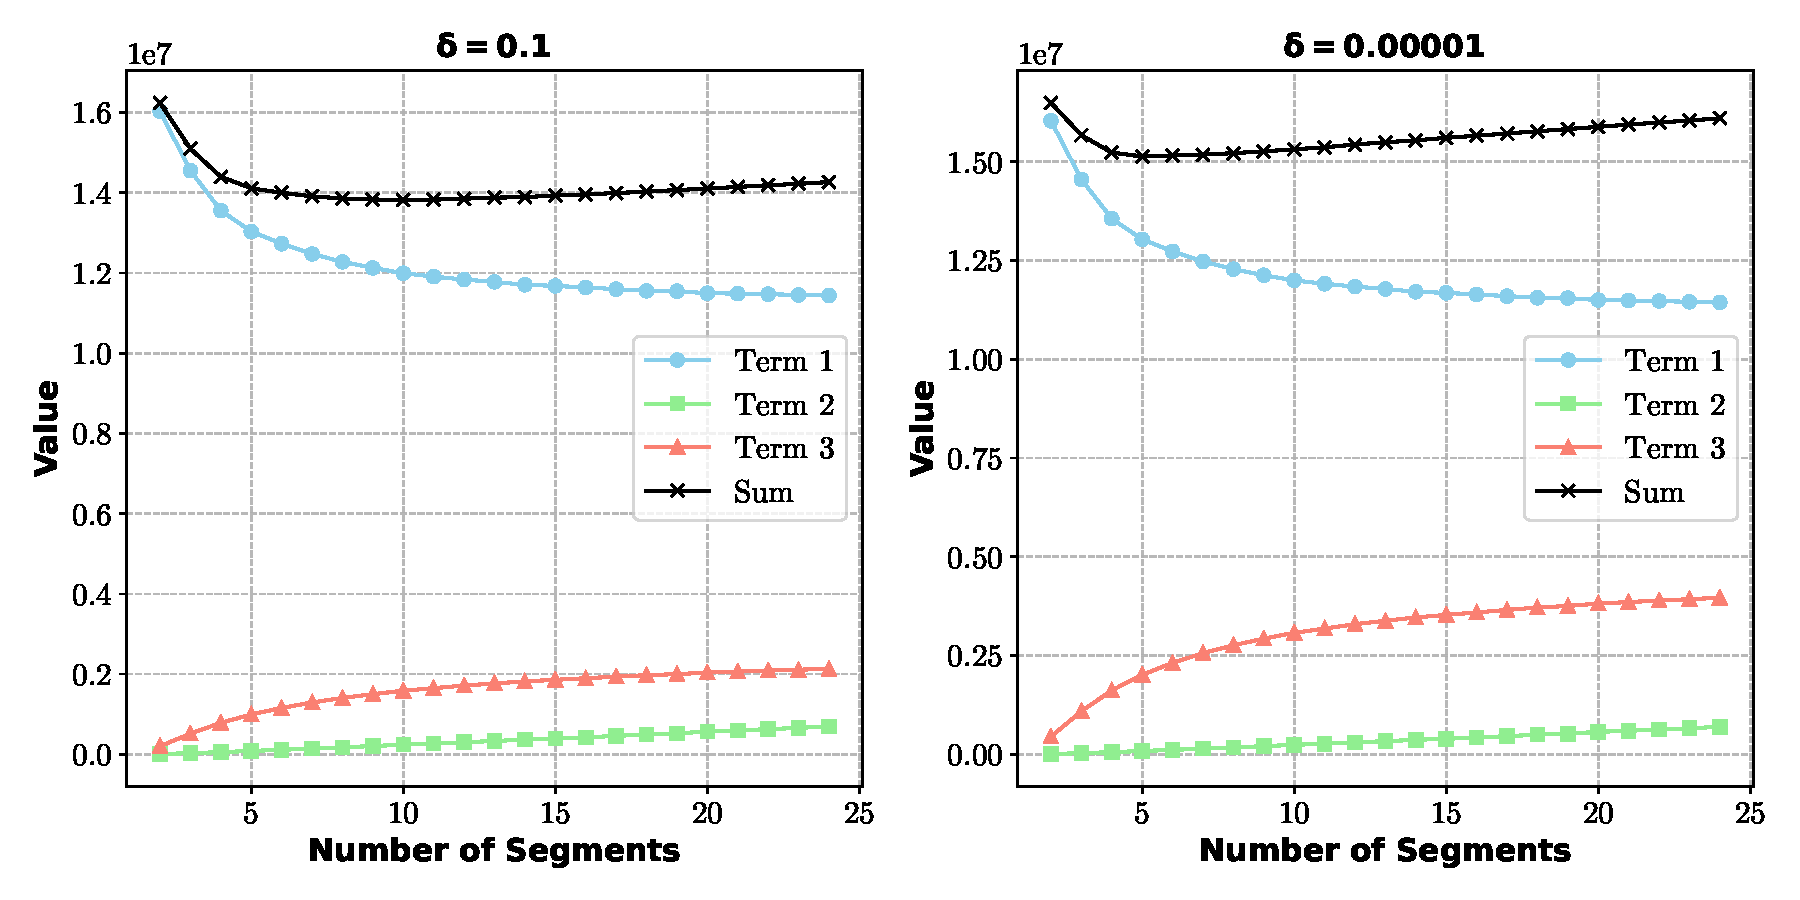
\includegraphics[width=0.55\textwidth]{Experiments_pdf/total_rate=50,T=200.pdf}
    \caption{Memory usage proportions under low arrival rate (total rate = 50, $T = 200$). Left: $\delta = 0.1$; Right: $\delta = 10^{-5}$.}
    \label{fig:fixed_T_200_rate_50_delta_0.1_1e-5}
\end{figure}

\begin{figure}[ht]
    \centering
    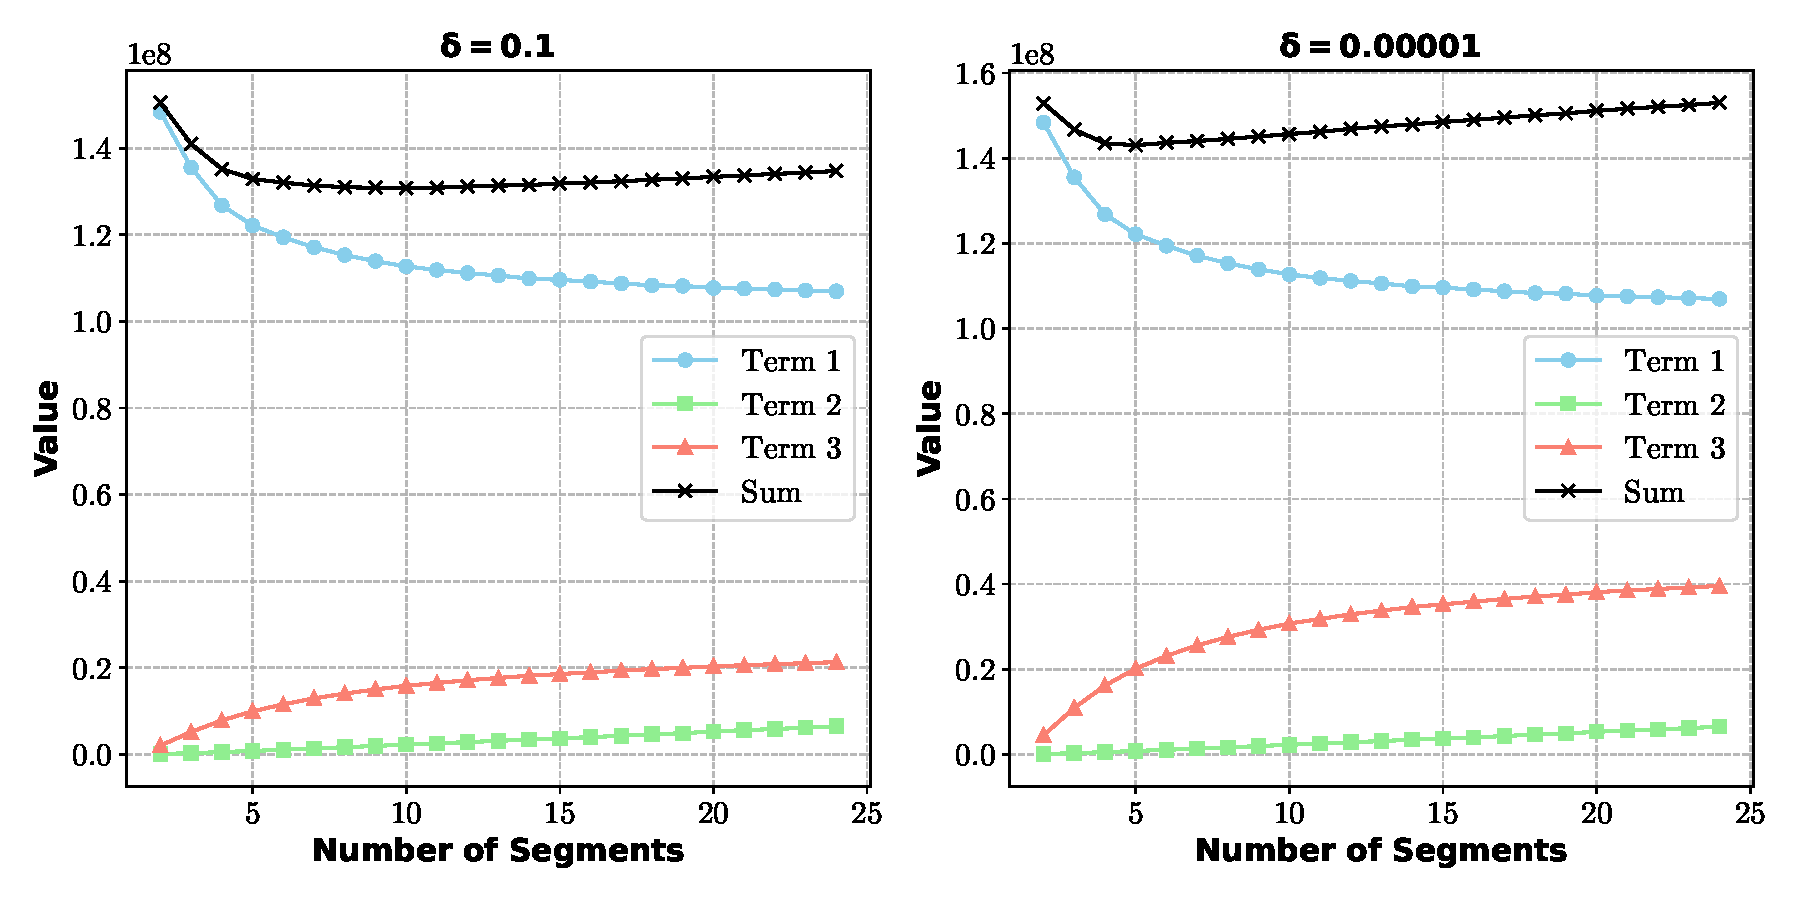
\includegraphics[width=0.55\textwidth]{Experiments_pdf/total_rate=500,T=200.pdf}
    \caption{Memory usage proportions under high arrival rate (total rate = 500, $T = 200$). Left: $\delta = 0.1$; Right: $\delta = 10^{-5}$.}
    \label{fig:fixed_T_200_rate_500_delta_0.1_1e-5}
\end{figure}

\begin{figure}[ht]
    \centering
    
\includegraphics[width=0.55\textwidth]{Experiments_pdf/total_rate=50,delta=0.001,T=20or2000.pdf}
    \caption{Memory usage proportions with varying time horizons (total rate = 50, $\delta = 0.001$). Left: $T = 20$; Right: $T = 2000$.}
    \label{fig:fixed_delta_0.001_rate_50_T_20_2000}
\end{figure}

These extensions demonstrate that the core threshold-based design, eviction prevention through controlled admission, remains robust to realistic deployment conditions. Time-varying arrival rates and segment-wise grouping introduce no fundamental barrier; the coupling-based analysis extends naturally with logarithmic overhead. Section~\ref{sec:experiments} illustrates this implementation on a real workload, where Nested WAIT uses coarser decode-stage segments rather than maintaining a separate threshold for every possible output length.

% \subsection{Optimality under arbitrary segments}
% \gan{Maybe this subsection should be put later.}
